\documentclass[12pt]{article}

\usepackage[utf8]{inputenc}

% Disable paragraph indentation
\usepackage{graphicx}

% For hyperlinks in figure captions
\usepackage{hyperref}

% Disable paragraph indentation
\setlength{\parindent}{0pt}

% Set the length of space between paragraphs
\setlength{\parskip}{12pt}

% Disable page numbering
\pagenumbering{gobble}

% For forcing figure position
\usepackage{float}


\title{Internet of Things - Homework - Question 10}
\author{Francesco Pastore 10629332}
\date{05-14-2024}

\begin{document}

\maketitle

\textbf{Question}

You have setup a weather monitoring station on your balcony and would like to transmit the acquired data over a web service (e.g., ThingSpeak).
You have no Wi-Fi connectivity at home, therefore you plan to use a long-range IoT communication technology.
After careful consideration, you need to choose between LoRa and NB-IoT

10. What are the main factors you would look at to make your final choice?

\textbf{Answer}

First, I would consider the coverage available in my area for LoRa and NB-IoT, as both technologies require a gateway to connect to the Internet.
While NB-IoT relies on the existing cellular network, LoRa requires a dedicated gateway in the area, which is not always available.

Looking at the coverage map for LoRa provided by The Things Network (Figure 1), it seems that there is only one gateway in my area, but it is far from my house.
The air distance is around 5 km (Figure 2), which is high but still within the generic range of LoRa considered as maximum 15 km.

On the other hand, due to the nature of NB-IoT, coverage is guaranteed by the cellular network and the many antennas available in the area.
I have used TIM's coverage map as an example (Figure 3), but other operators also have good coverage in my area.

If it is still possible to choose between the two technologies, I would consider the cost of the data plan required in the case of NB-IoT.
For example, I found a plan from ho.mobile (Figure 4) that offers 500MB of data for €2.99/month, which is a good deal for my use case.

For LoRa, some operators allow you to use the network for free, while others may require a subscription fee.
I wasn't able to find a specific plan for the LoRa gateway in my area, but I'd have to consider this factor when making my final choice.

In general, we also have to take into account that NB-IoT offers end-to-end security by default and it is more reliable than LoRa.

Ultimately, I would have to choose NB-IoT over LoRa for my use case because of the better coverage in my area.

\begin{figure}[H]
    \centering
    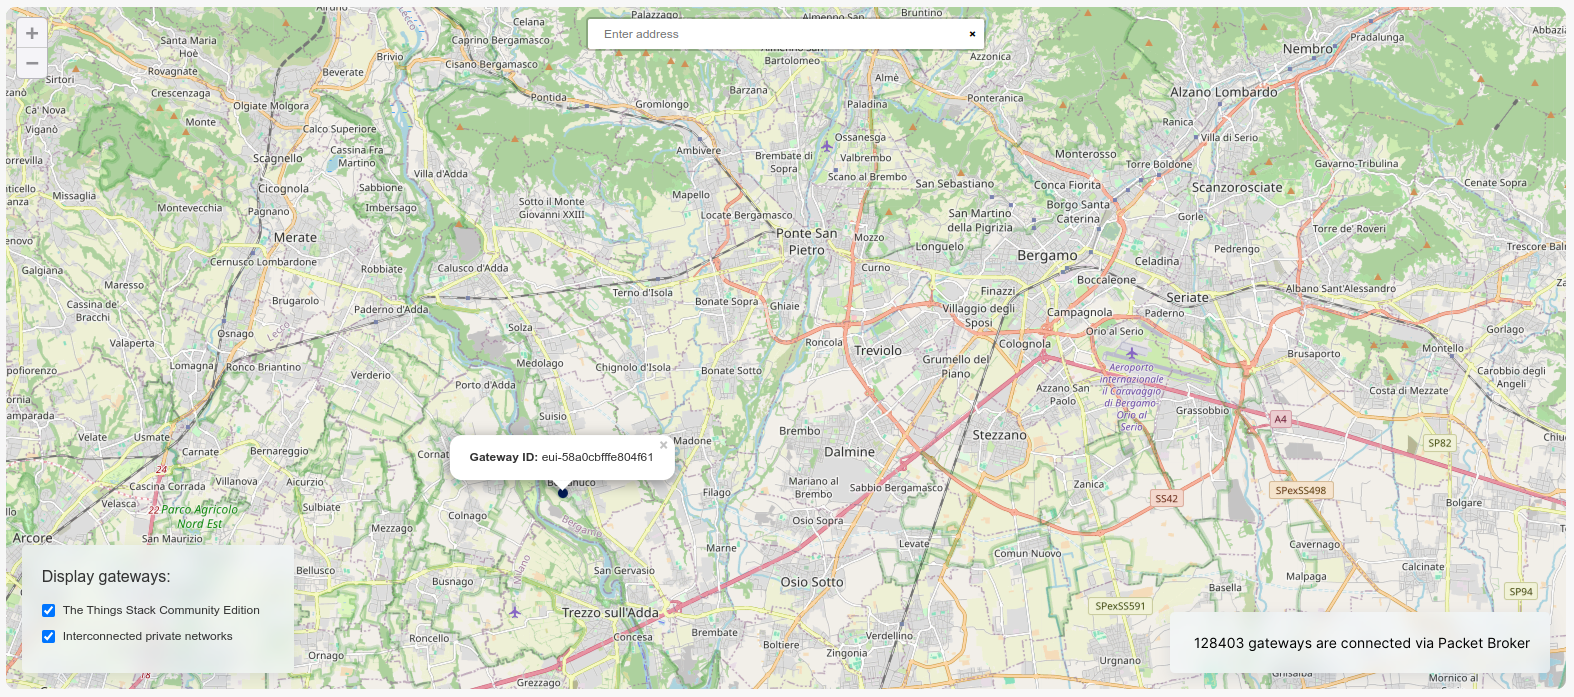
\includegraphics[width=0.8\textwidth]{./lora-coverage.png}
    \caption{LoRa coverage map in my area}
    \url{https://www.thethingsnetwork.org/map}
\end{figure}

\begin{figure}[H]
    \centering
    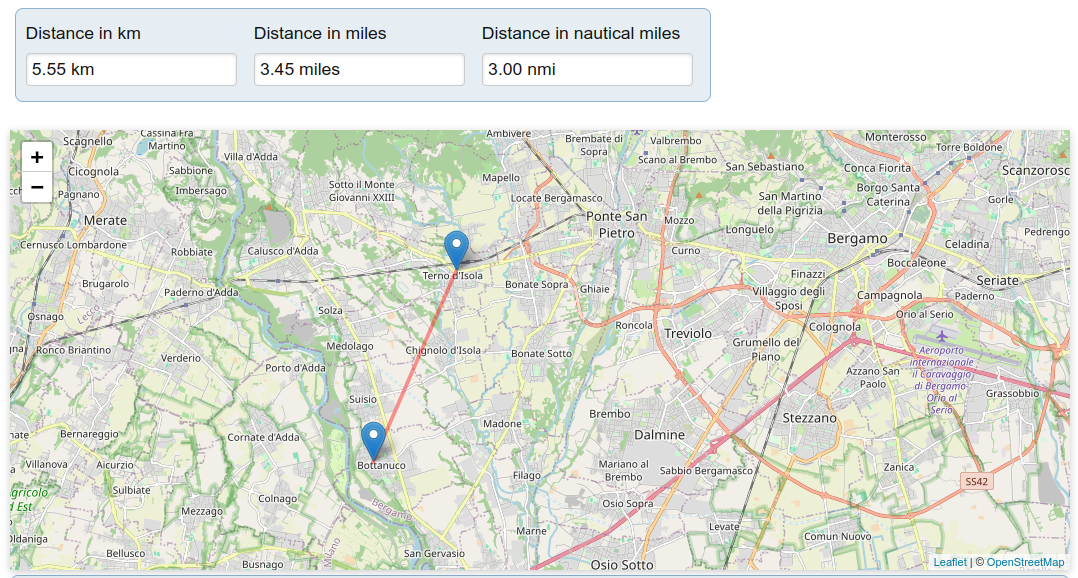
\includegraphics[width=0.8\textwidth]{./air-distance.png}
    \caption{Air distance between my house and the nearest LoRa gateway}
\end{figure}

\begin{figure}[H]
    \centering
    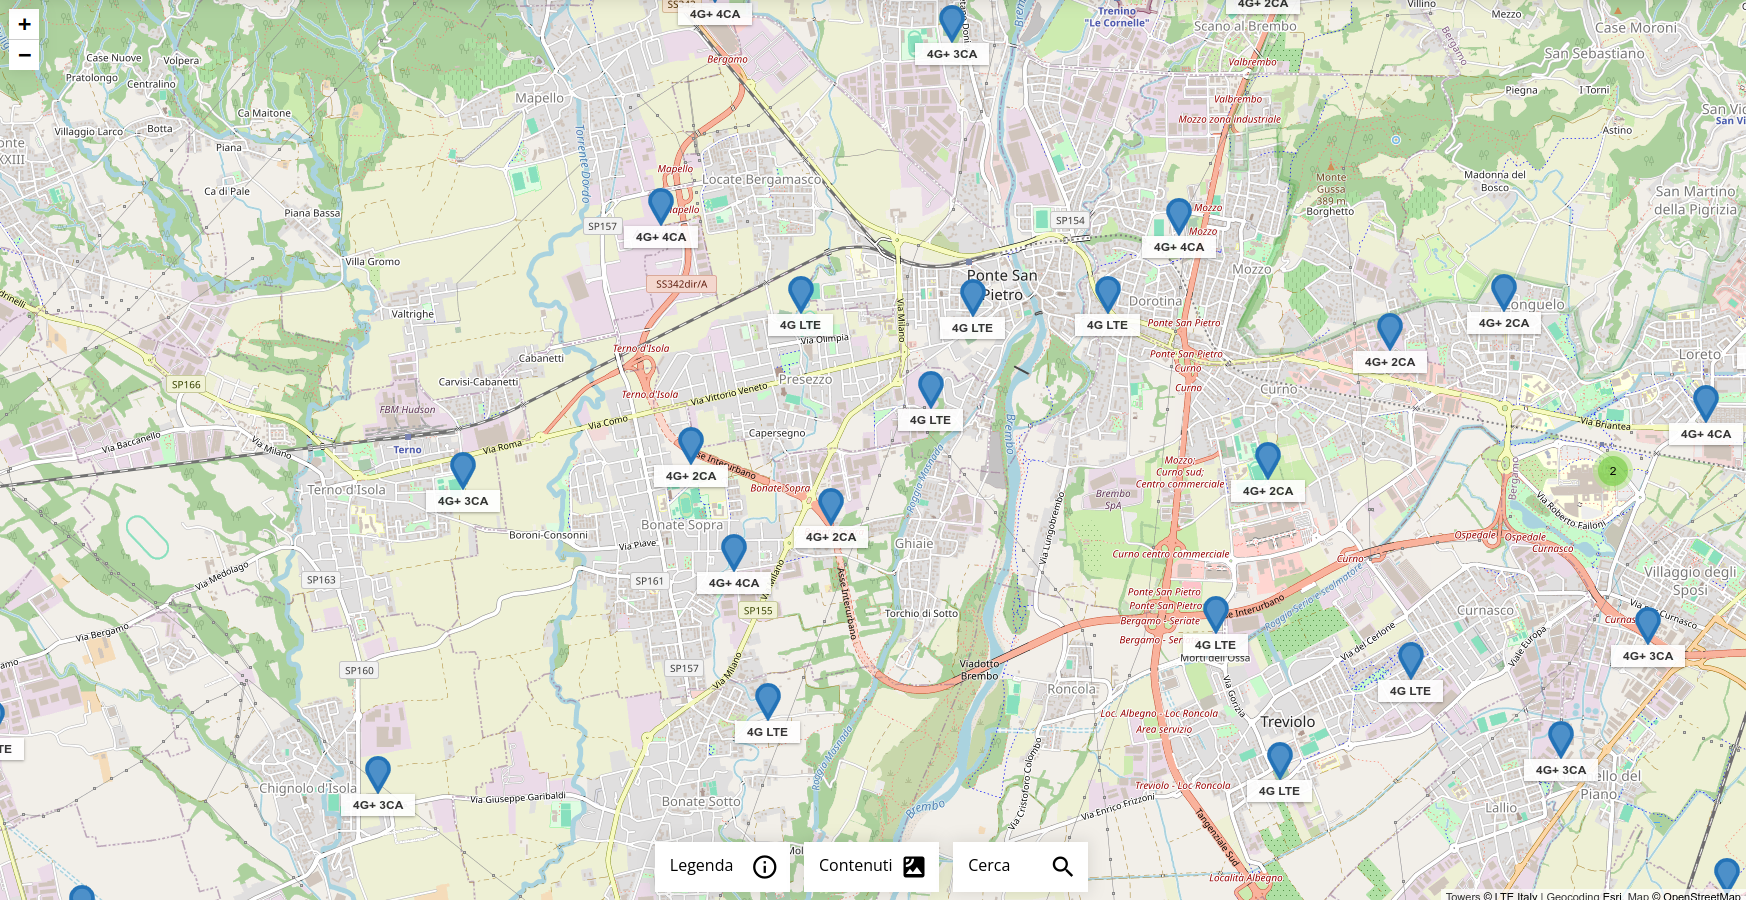
\includegraphics[width=0.8\textwidth]{./tim-coverage.png}
    \caption{TIM coverage map in my area}
    \url{https://lteitaly.it/it/public/map.php#14/45.690593/9.6017074}
\end{figure}


\begin{figure}[H]
    \centering
    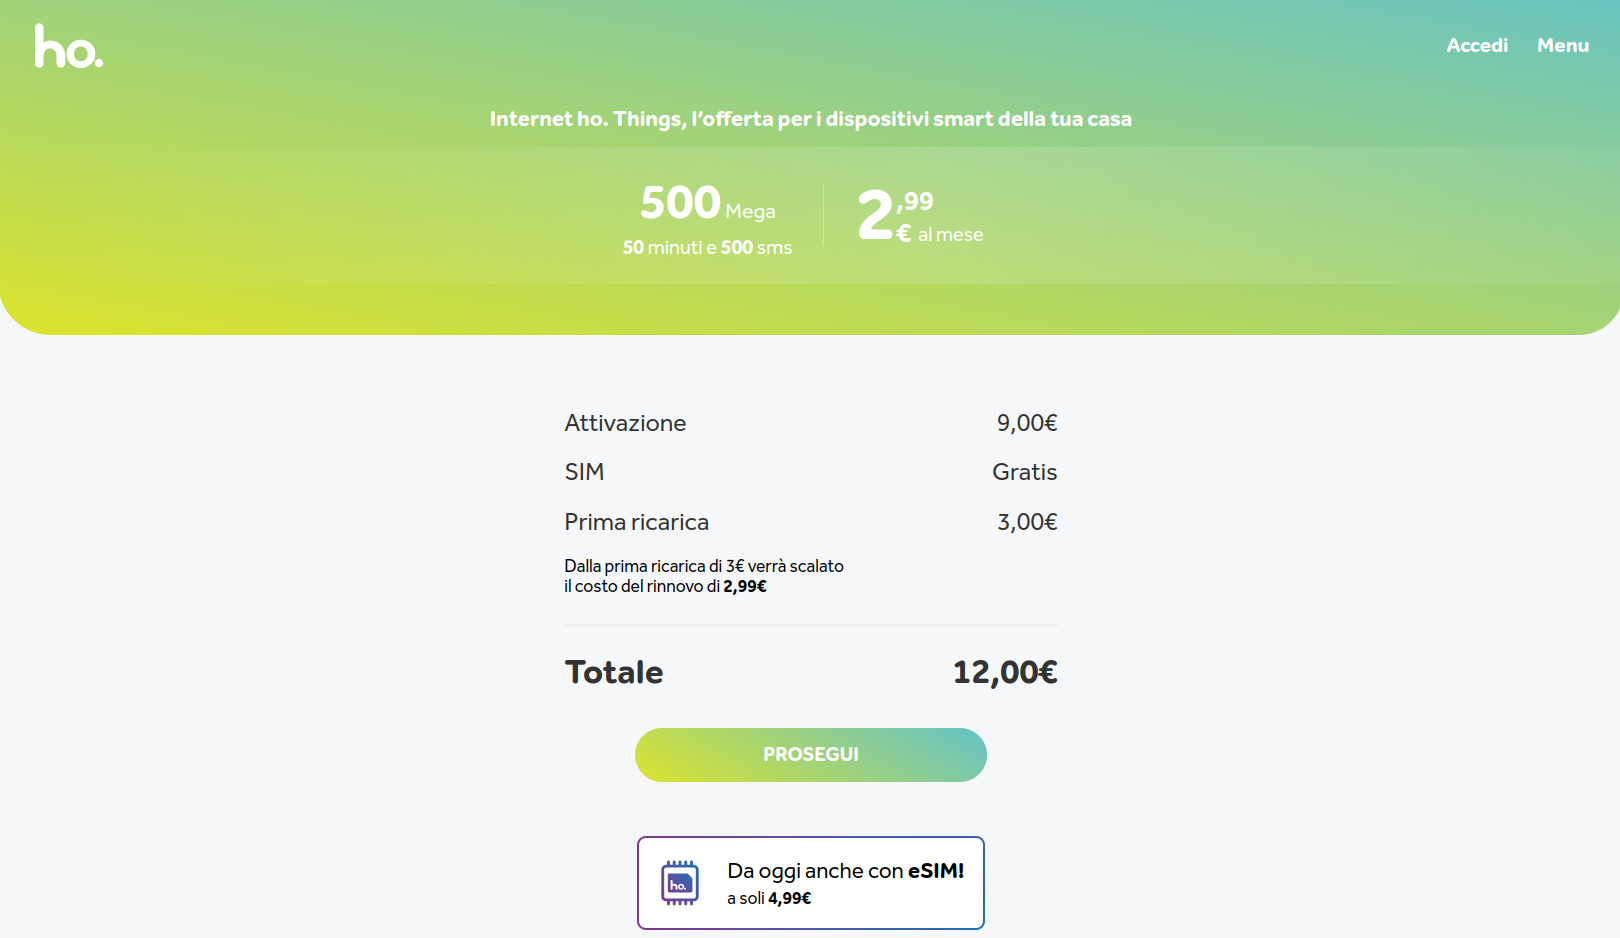
\includegraphics[width=0.8\textwidth]{./ho-sim.png}
    \caption{Example of SIM plan with ho.}
    \url{https://www.ho-mobile.it/ho-smarthome.html}
\end{figure}

\end{document}